\chapter{Coupled Cluster Theory}

The coupled cluster theory was developed by Fritz Coester and Hermann 
K\"ummel. It is a numerical technique used to describe many body systems. 
The method starts with a ground state Slater determinant, as the Slater determinant below, Eq. \ref{slaterdet}, corresponding to a system consisting of four particles.

\be
\frac{1}{4!}
\left|
\begin{array}{cccc}
\phi_i(x_1) & \phi_j(x_1) & \phi_k(x_1) & \phi_l(x_1)\\
\phi_i(x_2) & \phi_j(x_2) & \phi_k(x_2) & \phi_l(x_2)\\
\phi_i(x_3) & \phi_j(x_3) & \phi_k(x_3) & \phi_l(x_3)\\
\phi_i(x_4) & \phi_j(x_4) & \phi_k(x_4) & \phi_l(x_4)\\
\end{array}
\right|
\label{slaterdet}
\ee

A convenient shorthand notation for the Slater determinant consists of a 
Dirac-notation ket containing only the diagonal elements of the Slater 
determinant \cite{sjefer}.
The ket vector corresponding to Eq. \ref{slaterdet} would 
be 

\be
\ket{\phi_i( x_1)\phi_j(x_2)\phi_k( x_3) \phi_l( x_4)}.
\ee


When there are more orbitals available than particles occupying them, the 
ground state Slater determinant fails to account for the total state. 
The wavefunction would then be a linear combination of various Slater 
determinants where the other Slater determinants are excitations of the 
ground state.

The ansatz is that the total wavefunction can be written as

\be
\psi=e^T \phi_0 
\ee

where $T$, called the cluster operator, consists of cluster coefficients, which are to be determined via
the Schr\"odinger equation \cite{sjefer}.
The cluster operator is written in the form 

\be
T=T_1+T_2+T_3 + \cdots
\ee

$T_1$ is a operator of all single excitations, and $T_2$ the operator of 
all double excitations, and so on. 
By the formalism of the second quantization the excitation operators are expressed as 

\begin{align}
& T_1 = \sum_{ia} t^a_ia^\dagger_a a_i \\
& T_2 = \frac{1}{4} \sum_{ijab} t^{ab}_{ij} a^\dagger_aa^\dagger_ba_ja_i 
\end{align}

More generally an $n-$orbital cluster operator may be defined as %\cite{sjefer} 

\be
T_n = \left(\frac{1}{n!}\right)^2 \sum_{ij \dots ab \dots} t^{ab\dots}_{ij 
\dots} a^\dagger_aa^\dagger_b \dots a_ja_i 
\ee.

The energy expectation value is then computed by the relation 

\be
E = \bra{\phi_0}e^{-T}He^T \ket{\phi_0} 
\label{coupleenergy}
\ee

By using the Campbell-Baker-Hausdorff formula on $e^{-T}He^T$ Eq. \eqref{coupleenergy} transforms to

\be
E = \bra{\phi_0} H +[H,T_1] + [H,T_2] + \frac{1}{2}[[H,T_1],T_1]+ \frac{1}{2}[[H,T_2],T_2] + [[H,T_1],T_2] + \cdots \ket{\phi_0}.
\ee 

This expansion may appear more complicated than in Eq. \eqref{coupleenergy}. 
However there is an advantage with this new expansion, it terminates exactly
at four nested commutators when the Hamiltonian consists at most of a 
two-body term and at six nested commutators when three-body potentials are
present. 
%\cite{MortenogD.J.Dean}% Toward coupled cluster implementations in Nucl strct

The amplitudes $t_i^a$ etc, can be found by the equations

\begin{equation}
\begin{split}
& \bra{\phi^a_i}e^{-T}He^T\ket{\phi_0}=0\\
& \bra{\phi^{ab}_{ij}}e^{-T}He^T\ket{\phi_0}=0
\end{split}
\label{cclikn}
\end{equation}
In this work the cluster operator is truncated at $T_2$, the equations in Eq. 
\eqref{cclikn} are then the 
only equations needed to determine the cluster amplitudes $t^a_i$ and $t^{ab}_{ij}$.\\

\section{The CCSD energy equation}

The energy problem simplifies a lot when the normalized Hamiltonian, according to the quasiparticle formalism, is used. When our Hamiltonian is at most
a two particle operator, the exact expression will be truncated at

\be
\begin{split}
& e^{-T} H_Ne^T =H_N +[H_N,T_1] + [H_N,T_2] +\\
& \frac{1}{2}[[H_N,T_1],T_1]+ \frac{1}{2}[[H_N,T_2],T_2] + [[H_N,T_1],T_2] 
\label{hausd}
\end{split}
\ee

Where 

\be
H_N=\sum_{\alpha\beta}f_{\alpha\beta}N(a^\dagger_\alpha a_\beta)+
\frac{1}{4}\sum_{\alpha\beta\gamma\delta}V_{\alpha\beta\gamma\delta}N(
a^\dagger_\alpha a^\dagger_\beta a_\delta a_\gamma).
\label{normha}
\ee

%When the expectation value of this expression is computed, only three terms
%will survive.

%Since the expression for the normalized Hamiltonian is already calculated in
%Eq. \eqref{normalham} and given again in Eq. \eqref{normha}.

By taking the expectation value of the expanded Hamiltonian, 
Eq. \eqref{hausd},
 we see that the first term doesn't contribute.\\
I will now go thoroughly through the anti commutators.
I start with the anti commutator of $H_1$ and $T_1$. 
\be
\{H_N,T_1\}=H_NT_1+T_1H_N
\ee

Let us first calculate $\bra{\Phi_0}H_NT_1\ket{\Phi_0}$, 

\be
\begin{split}
&\sum_{\substack{\alpha\beta\gamma\delta,\\ i\in holes,\\ a\in particles}}
 f_{\alpha\beta}t^a_i\bra{\Phi_0}\wick{21}{<1a^\dagger_\alpha<2 a_\beta
>2a^\dagger_a >1a_i}\ket{\Phi_0}+V_{\alpha\beta\gamma\delta}t^{a}_{i}
\sum_{all \, contractions}\bra{\Phi_0}{a^\dagger_\alpha a^\dagger_\beta a_\delta a_\gamma 
a^\dagger_a a_i}\ket{\Phi_0}\\
&=\sum_{\substack{a \in particles,\\ i \in holes}}f_{ia}t^a_i.
\end{split}
\ee

The term $\bra{\Phi_0}T_1H_N\ket{\Phi_0}$ is zero.

%\be
%\bra{\Phi_0}T_1H_N\ket{\Phi_0}=0
%\ee

All the terms with a cluster operator to the left of the normalized Hamiltonian
become zero when taking the expectation value. By using these relations, we can  write down the energy equation to a somewhat less tedious form.

\be
E=\bra{\Phi_0}H_N+H_NT_1+H_NT_2+\frac{1}{2}H_NT^2_1+\dots \ket{\Phi_0}
\label{lastformham}
\ee

The other terms to calculate 
are 

\be
\begin{split}
& H_NT_2 \\
& \frac{1}{2}H_NT_1^2
\label{lasttwo}
\end{split}
\ee

Since the other terms in Eq. \eqref{lastformham} will be zero, for calculations of the non contributing terms, I will again refer to \cite{sjefer}.\\

For the terms in Eq. \eqref{lasttwo} it's only the two particle operator of
the Hamiltonian that contributes.

The first term to be considered is $H_NT_2$

\be
\begin{split}
&\bra{\Phi_0}H_NT_2\ket{\Phi_0}=\frac{1}{16}\big(\sum_{\substack{\alpha\beta\gamma\delta,\\ab \in particles\\ij\in holes}}
V_{\alpha\beta\gamma\delta}t^{ab}_{ij}\bra{\Phi_0}\wick{4321}{<1a^\dagger_\alpha 
<2a^\dagger_\beta <3a_\delta <4a_\gamma >4a^\dagger_a >3a^\dagger_b >2a_j >1a_i }
\ket{\Phi_0}\\
&+V_{\alpha\beta\gamma\delta}t^{ab}_{ij}\bra{\Phi_0}\wick{4321}{<1a^\dagger_\alpha <2a^\dagger_\beta <3a_\delta <4a_\gamma >4a^\dagger_a >3a^\dagger_b 
>1a_j >2a_i} \ket{\Phi_0}
+V_{\alpha\beta\gamma\delta}t^{ab}_{ij}\bra{\Phi_0}\wick{4321}{<1a^\dagger_\alpha 
<2a^\dagger_\beta <4a_\delta <3a_\gamma >4a^\dagger_a >3a^\dagger_b >2a_j >1a_i }
\ket{\Phi_0}\\
&+V_{\alpha\beta\gamma\delta}t^{ab}_{ij}\bra{\Phi_0}\wick{4321}{<1a^\dagger_\alpha 
<2a^\dagger_\beta <4a_\delta <3a_\gamma >4a^\dagger_a >3a^\dagger_b >1a_j >2a_i }
\ket{\Phi_0}\big)\\
&= \frac{1}{4}\sum_{\substack{ab \in particles \\ij \in holes}} V_{ijab}
t^{ab}_{ij}
\end{split}
\ee

The last expectation value is calculated by the same method,

\be
\frac{1}{2}\bra{\Phi_0}H_NT_1^2\ket{\Phi_0}=\frac{1}{2}
\sum_{\substack{a,b\in particles,\\i,j \in holes}} V_{ijab}t^a_it^b_j.
\ee

We sum the terms contributing to the energy, in the coupled cluster 
single and doubly excited approximation, CCSD;

\be
E_{CC}=E_{CCSD}-E_0=\sum_{\substack{i, a}}f_{ia}t^a_i +  \frac{1}{4}\sum_{\substack{i,j \\a,b}} V_{ijab}t^{ab}_{ij}+
\frac{1}{2}\sum_{\substack{i,j,\\a,b }} V_{ijab}t^a_it^
b_j.
\label{ECCSD}
\ee 
Where $i,j$ act only in the hole space and $a,b$ act in the particle 
space.\\  
This energy relation is valid even if the cluster operator is not truncated 
at $T_2$, when  the Hamiltonian is a twobody operator. The cluster operators 
such as $T_3$ would contribute indirectly through the amplitude equations.

\section{The CCSD amplitude equations}

The amplitude equations in Eq. \eqref{cclikn}, has to be solved to compute 
the energy. % When truncating after $T_2$, the CCSD approximation, these two
%are the only one to solve.
The single excitation amplitudes $t^a_i$ is
computed from Eq.\eqref{baret1}.

\be
\bra{\Phi^a_i}e^{-T}He^T\ket{\Phi_0}.
\label{baret1}
\ee

The double excitation amplitude, $t^{ab}_{ij}$, is determined from
Eq.\eqref{baret2}.

\be
\bra{\Phi^{ab}_{ij}}e^{-T}He^T\ket{\Phi_0}.
\label{baret2}
\ee

Computing these ones is much more tedious, and will require much more terms
than the energy problem since they are not an expectation value of the 
reference vacuum, but they combine an excited state and the vacuum state. 
There are more creation and destruction operators to handle. The singly 
excited state is written as

\be
\bra{\Phi^a_i}=\bra{\Phi_0}a^\dagger_i a_a
\ee

The leading term in the equation for the singly excited state is just $H$. 
Only the one particle part of the Hamiltonian contributes to the first 
leading term of the singly excited amplitude, $\bra{\Phi^a_i}e^{-T}He^T\ket{\Phi_0}.$

\be
\bra{\Phi^a_i}=\bra{\Phi_0}a^\dagger_i a_ae^{-T}He^T\ket{\Phi_0}=f_{ai}
\ee

The first leading term in $\bra{\Phi^{ab}_{ij}}e^{-T}He^T\ket{\Phi_0}$ is 

\be
\bra{\Phi_0}a^\dagger_ia^\dagger_j a_ba_ae^{-T}He^T\ket{\Phi_0}=V_{abij}. 
\ee\\

The tedious work arises when
trying to calculate parts including the cluster operators. 
Doing the entire calculations would be to boring to follow for the
reader, since they are already calculated in other papers, it will be skipped. 
However the interested reader may take a look at \cite{sjefer}.

The resulting equation for the $T_1$ amplitude is

\be
\begin{split}
& 0=f_{ai}+\sum_cf_{ac}t^c_i-\sum_kf_{ki}t^a_k+\sum_{kc}\bra{ka}V\ket{ci}t^c_k+
\sum_{kc}f_{kc}t^{ac}_{ik}+\frac{1}{2}\sum\bra{ka}V\ket{cd}t^{cd}_{ki}-\\
&\frac{1}{2}\sum_{klc}\bra{kl}V\ket{ci}t^{ca}_{kl}-\sum_{kc}f_{kc}t^c_it^a_k-
\sum_{klc}\bra{kl}V\ket{ci}t^c_kt^a_l+\sum_{kcd}\bra{ka}V\ket{cd}t^c_kt^d_i-\\
&\sum_{klcd}\bra{kl}V\ket{cd}t^c_kt^d_it^a_l+\sum_{klcd}\bra{kl}V\ket{cd}t^c_kt^{da}_{li}-\frac{1}{2}\sum_{klcd}\bra{kl}V\ket{cd}t^{cd}_{ki}t^a_l-
\frac{1}{2}\sum_{klcd}\bra{kl}V\ket{cd}t^{ca}_{kl}t^d_i
\label{firstamplitude}
\end{split}
\ee

While the amplitude equation for $T_2$ is

\be
\begin{split}
& 0= \bra{ab}V\ket{ij}+\sum_c(f_{bc}t^{ac}_{ij}-f_{ac}t^{bc}_{ij})-\sum_k(f_{kj}
t^{ab}_{ik}-f_{ki}t^{ab}_{jk})+\\
& \frac{1}{2}\sum_{kl}\bra{kl}V\ket{ij}t^{ab}_{kl}+\frac{1}{2}\sum_{cd}\bra{
ab}V\ket{cd}t^{cd}_{ij}+P(ij)P(ab)\sum_{kc}\bra{kb}V\ket{cj}t^{ac}_{ik}+\\
& P(ij)\sum_c\bra{ab}V\ket{cj}t^c_i-P(ab)\sum_k\bra{kb}V\ket{ij}t^a_k+\\
& \frac{1}{2}P(ij)P(ab)\sum_{klcd}\bra{kl}V\ket{cd}t^{ac}_{ik}t^{db}_{lj}+
\frac{1}{4}\sum_{klcd}\bra{kl}V\ket{cd}t^{cd}_{ij}t^{ab}_{kl}-\\
&P(ab)\frac{1}{2}\sum_{kl}\bra{kl}V\ket{cd}t^{ac}_{ij}t^{bd}_{kl}-P(ij)\frac{1}{2}\sum_{klcd}\bra{kl}V\ket{cd}t^{ab}_{ik}t^{cd}_{jl}+\\
& P(ab)\frac{1}{2}\sum_{kl}\bra{kl}V\ket{ij}t^a_kt^b_l+P(ij)\frac{1}{2}\sum_{cd}\bra{ab}V\ket{cd}t^c_it^d_j-P(ij)P(ab)\sum_{kc}\bra{kb}V\ket{ic}t^a_kt^c_j+\\
& P(ab)\sum_{kc}f_{kc}t^a_kt^{bc}_{ij}+P(ij)\sum_{kc}f_{kc}t^c_it^{ab}_{jk}-\\
& P(ij)\sum_{klc}\bra{kl}V\ket{ci}t^c_kt^{ab}_{lj}+P(ab)\sum_{kcd}\bra{ka}V\ket{cd}t^c_kt^{db}_{ij}+ \\
& P(ij)P(ab)\sum_{kcd}\bra{ak}V\ket{dc}t^d_it^{bc}_{jk}+P(ij)P(ab)\sum_{klc}\bra{kl}V\ket{ic}t^a_lt^{bc}_{jk}+\\
& P(ij)\frac{1}{2}\sum_{klc}\bra{kl}V\ket{cj}t^c_it^{ab}_{kl}-P(ab)\frac{1}{2}\sum_{kcd}\bra{kb}V\ket{cd}t^a_kt^{cd}_{ij}-\\
& P(ij)P(ab)\frac{1}{2}\sum_{kcd}\bra{kb}V\ket{cd}t^c_it^a_kt^d_j+P(ij)P(ab)\frac{1}{2}\sum_{klc}\bra{kl}V\ket{cj}t^c_it^a_kt^{b}_{l}-\\
& P(ij)\sum_{klcd}\bra{kl}V\ket{cd}t^c_kt^d_it^{ab}_{lj}-P(ab)\sum_{klcd}\bra{kl}V\ket{cd}t^c_kt^a_lt^{db}_{ij}+\\
& P(ij)\frac{1}{4}\sum_{klcd}\bra{kl}V\ket{cd}t^c_it^d_jt^{ab}_{kl}+P(ab)\frac{1}{4}\sum_{klcd}\bra{kl}V\ket{cd}t^a_kt^b_lt^{cd}_{ij}+\\
& P(ij)P(ab)\sum_{klcd}\bra{kl}V\ket{cd}t^c_it^b_lt^{ad}_{kj}+P(ij)P(ab)\frac{1}{4}\sum_{klcd}\bra{kl}V\ket{cd}t^c_it^a_kt^d_jt^b_l.
\label{secondamplitude}
\end{split}
\ee 

The notation $P(ab)$ indicates a permutation operator whose action on a function, $f,$  is defined as

\be
P(pq)f(p,q)=f(p,q)-f(q,p)
\ee


\section{Coupled cluster diagrams}

As a relief there exists easier ways to construct the coupled 
cluster energy and amplitude equations, that is with a diagrammatic
approach. The equations can be represented by some sort of Feynman
diagrams, the rules are not quite the same as in ordinary many body
physics, somehow distorted because of the cluster operators. 
New rules are needed, and they are as follow

\begin{enumerate}
\item As in ordinary many body perturbation, holes are represented 
by downward pointing lines and particles by upward pointing lines.

\begin{figure}[htp]
\centering
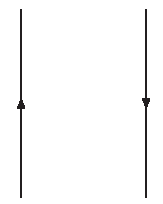
\includegraphics[scale=0.75]{holepart}
\caption{Diagrammatic representation of holes and particles, holes 
with an downward pointing arrow and particles with and upward pointing arrow.}
\label{holepart}
\end{figure}

\item The reference wavefunction, $\Phi_0,$ is represented by empty
 space.

\item Dynamical operators such as the one particle and two particle
part of the Hamiltonian are depicted by horizontal dashed lines.

\item The cluster operators are depicted by solid horizontal lines.

\item The one particle component of the Hamiltonian is represented
by a dashed interaction line capped by an $X.$


\item Representation of the cluster operators is seen in 
Fig (\ref{clusterdi}). In the diagram representing the $T_1$ amplitude there
is one incoming hole line and one outgoing particle line meeting at a solid
horizontal line.


\begin{figure}[htp]
\centering
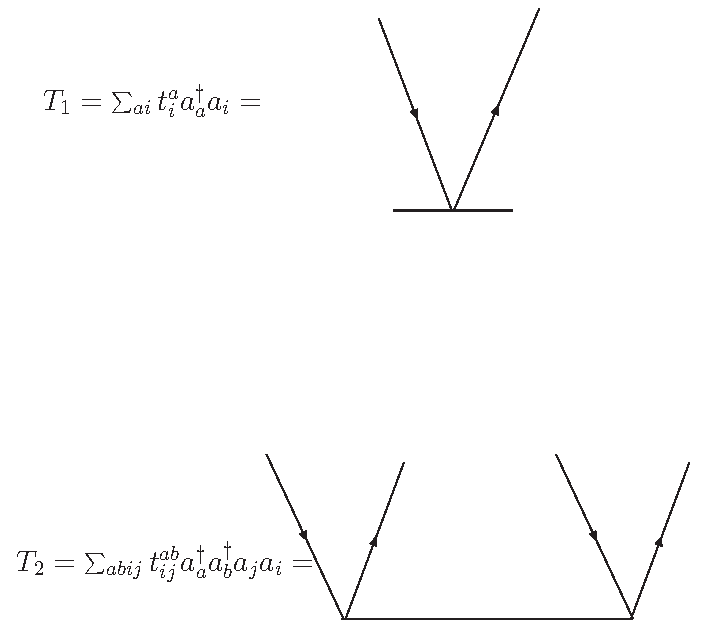
\includegraphics[scale=0.5]{clusterop}
\caption{Diagrammatic representation of the cluster operators $T_1$
and $T_2$.}
\label{clusterdi}
\end{figure}

The diagram representing $T_2$ consists of two incoming hole lines and two
outgoing particle lines. 


\item For each hole line, multiply with a factor of -1.

\item For each loop, multiply with a factor of -1

\item If there are $n$ equivalent vertices's in the diagram, multiply
with the factor $\frac{1}{n!}.$

\item For each pair of unique external hole or particle lines, multiply with
 the permutation operator $P(pq).$


\end{enumerate}

By using the above diagram rules it is possible to write diagrams
corresponding to the energy equation and amplitude equations. 

Like the diagrams for the energy equation in Eq. \eqref{lastformham}, 

\be
E=\bra{\Phi_0}H_N+H_NT_1+H_Nt_2+\frac{1}{2}H_NT^2_1+\dots \ket{\Phi_0}
\ee

can be evaluated with the above rules. The first term will not
contribute since the operator is normalized and therefore will
annihilate the vacuum state and give zero contribution.

Lets now study the second term


\be
\bra{\Phi_0}H_NT_1\ket{\Phi_0}
\label{firstendi}
\ee


Since both the incoming and outgoing states are the same there
should be now external lines, meaning that there shouldn't be 
any lines neither below or above the two horizontal operator 
lines. The $T_1$ operator stands to the right, and it's 
corresponding interaction line should then be in the bottom of 
the diagram. Only the one particle operator contributes since with a two 
particle operator it is impossible to draw a diagram with just internal 
lines. See Fig. (\ref{firstenedi}). 

%Fig. (\ref{firstenedi}) shows the diagrammatic representation of
%the energy term $\bra{\Phi_0}H_NT_1\ket{\Phi_0}.$
%Eq. \eqref{firstendi}

\begin{figure}[htp]
\centering
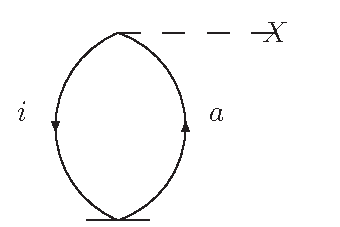
\includegraphics[scale=0.75]{firstenedi}
\caption{Diagrammatic representation of the first term in the 
ECCSD energy equation.}
\label{firstenedi}
\end{figure}






The second contributing part

\be
\bra{\Phi_0}H_NT_2\ket{\Phi_0},
\label{secendi}
\ee

has also the same ingoing as outgoing state, the same 
reasoning, with none external lines still yields. Since the 
cluster operator is the rightmost one, the interaction line 
representing it should again be at the bottom. However to this 
part only the two-particle operator of the Hamiltonian is 
contributing, something which should be reflected in the 
diagram. Fig. \ref{secndi} shows the diagram representing Eq. 
\eqref{secendi}.

\begin{figure}[htp]
\centering
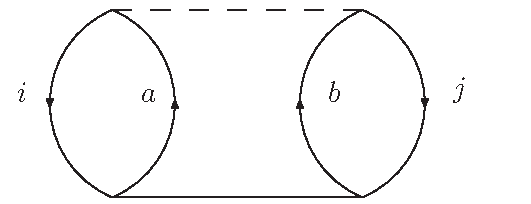
\includegraphics[scale=0.75]{secenedi}
\caption{Diagrammatic representation of the second term in the 
ECCSD energy equation.}
\label{secndi}
\end{figure}

The last part contributing to the $ECCSD$ energy equation is the
term 

\be
\frac{1}{2}\bra{\Phi_0}H_NT_1^2\ket{\Phi_0}
\label{thirdpartendi}
\ee

The interaction lines corresponding to the two cluster operators
will again have to be drawn at the bottom of the diagram, the 
difference in this diagram, Fig. (\ref{thirdenedi}), from 
Fig. (\ref{secndi}) is that the 
interaction line corresponding to the cluster operator is 
split since there are two one excitation cluster operators to
the right in Eq. \eqref{thirdpartendi} 

\begin{figure}[htp]
\centering
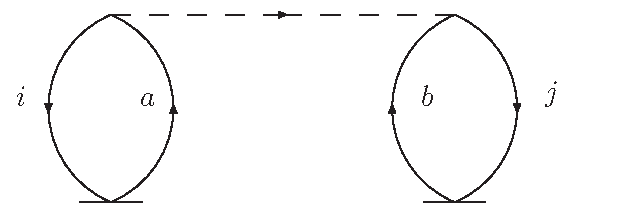
\includegraphics[scale=0.75]{thirdenedi}
\caption{Diagrammatic representation of the last term in the 
ECCSD energy equation.}
\label{thirdenedi}
\end{figure}

The cluster diagrams is computed by the same reasoning, keeping in mind that
for the $T1$ equation there should be one incoming hole line and one outgoing
particle line. The diagrams corresponding to the $T2$ equation all have two
incoming hole lines and two outgoing particle lines. The first leading term 
in the equation corresponding to $T1$ consists just of the Hamiltonian, and 
only the one particle part of it contributes. It's corresponding diagram is
depicted in Fig. (\ref{firstamplt1}).  


\begin{figure}[htp]
\centering
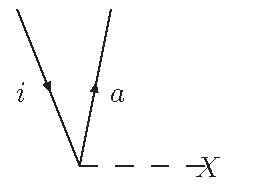
\includegraphics[scale=0.75]{firstampl}
\caption{The diagram representing the first leading term in the
$T_1$ amplitude equation.}
\label{firstamplt1}
\end{figure}

The other diagrams corresponding to $T1$ is made with the same reasoning. 
All diagrams contributing to the $T_1$ equation can be seen in Fig. (\ref{t1_eqn_diag}).\\


\begin{figure}[htp]
\centering
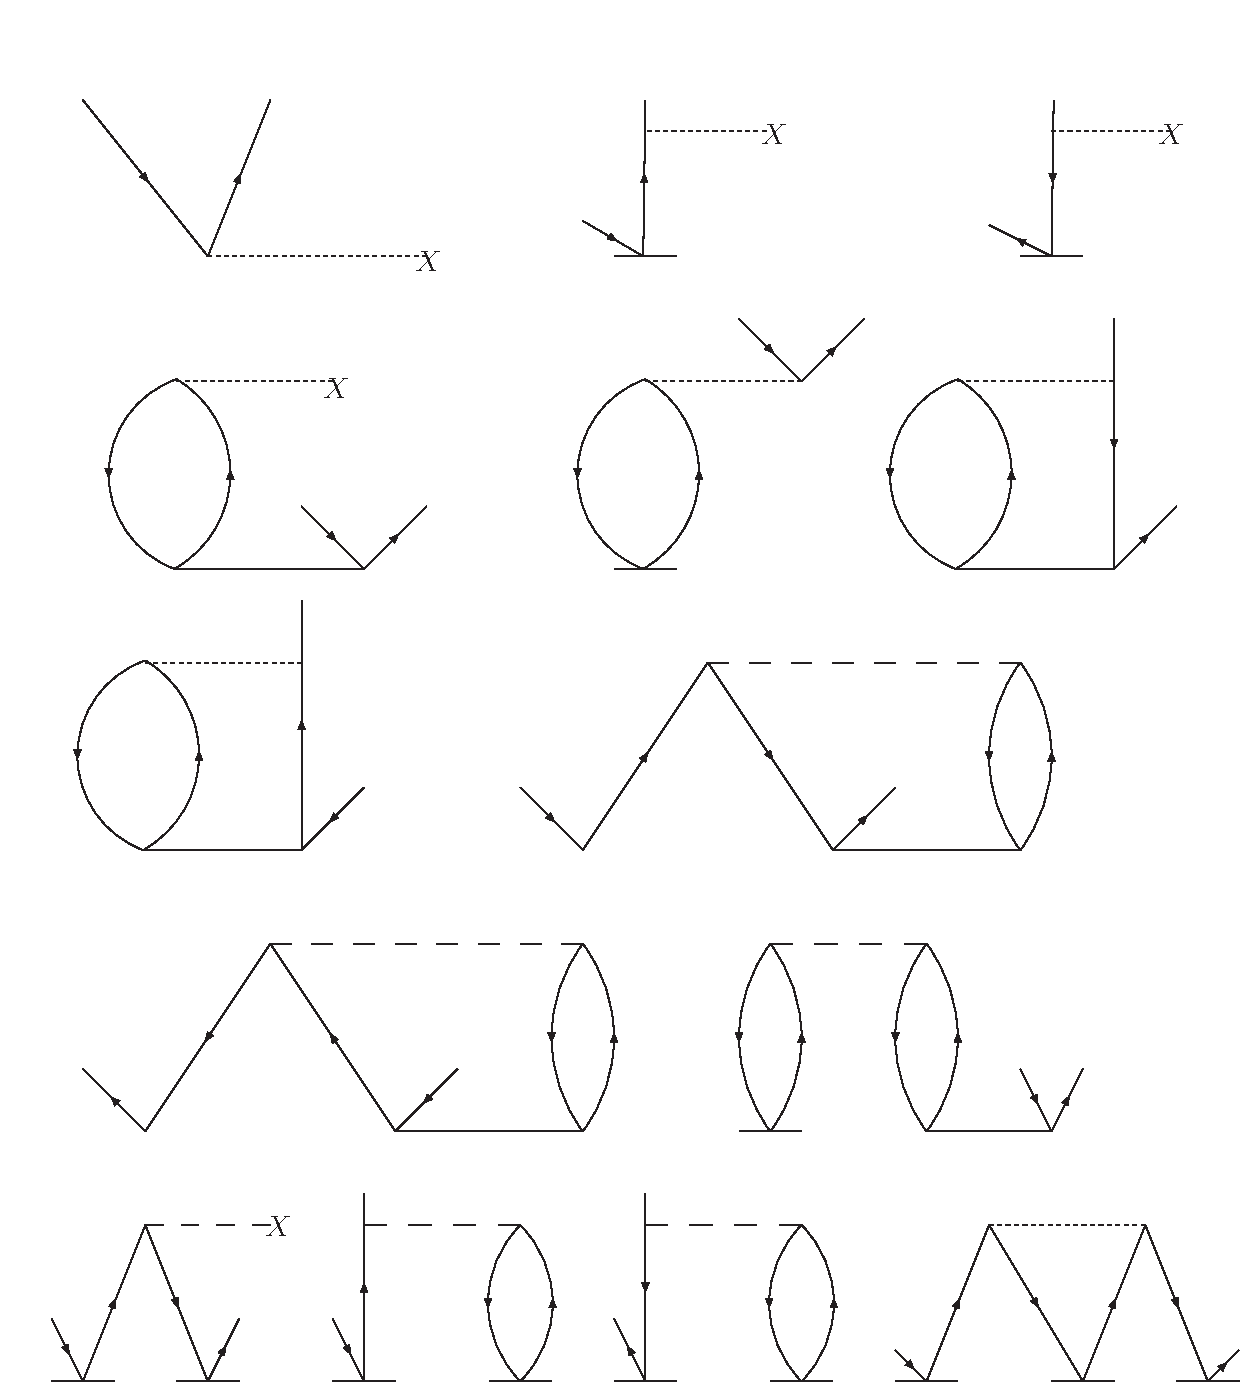
\includegraphics[scale=0.5]{t1_eqn_diag}
\caption{All diagrams contributing to the equation for solving the
$T_1$ amplitude.}
\label{t1_eqn_diag}
\end{figure}

%\clearpage

In the $T2$ amplitude diagrams there should be two incoming hole lines and
two outgoing particle lines. The first leading term consists just of the 
twoparticle operator. All the diagrams contributing to $T2$ are depicted in 
Fig. (\ref{t2_eqn_diag}).
\clearpage

\begin{figure}[htp]
\centering
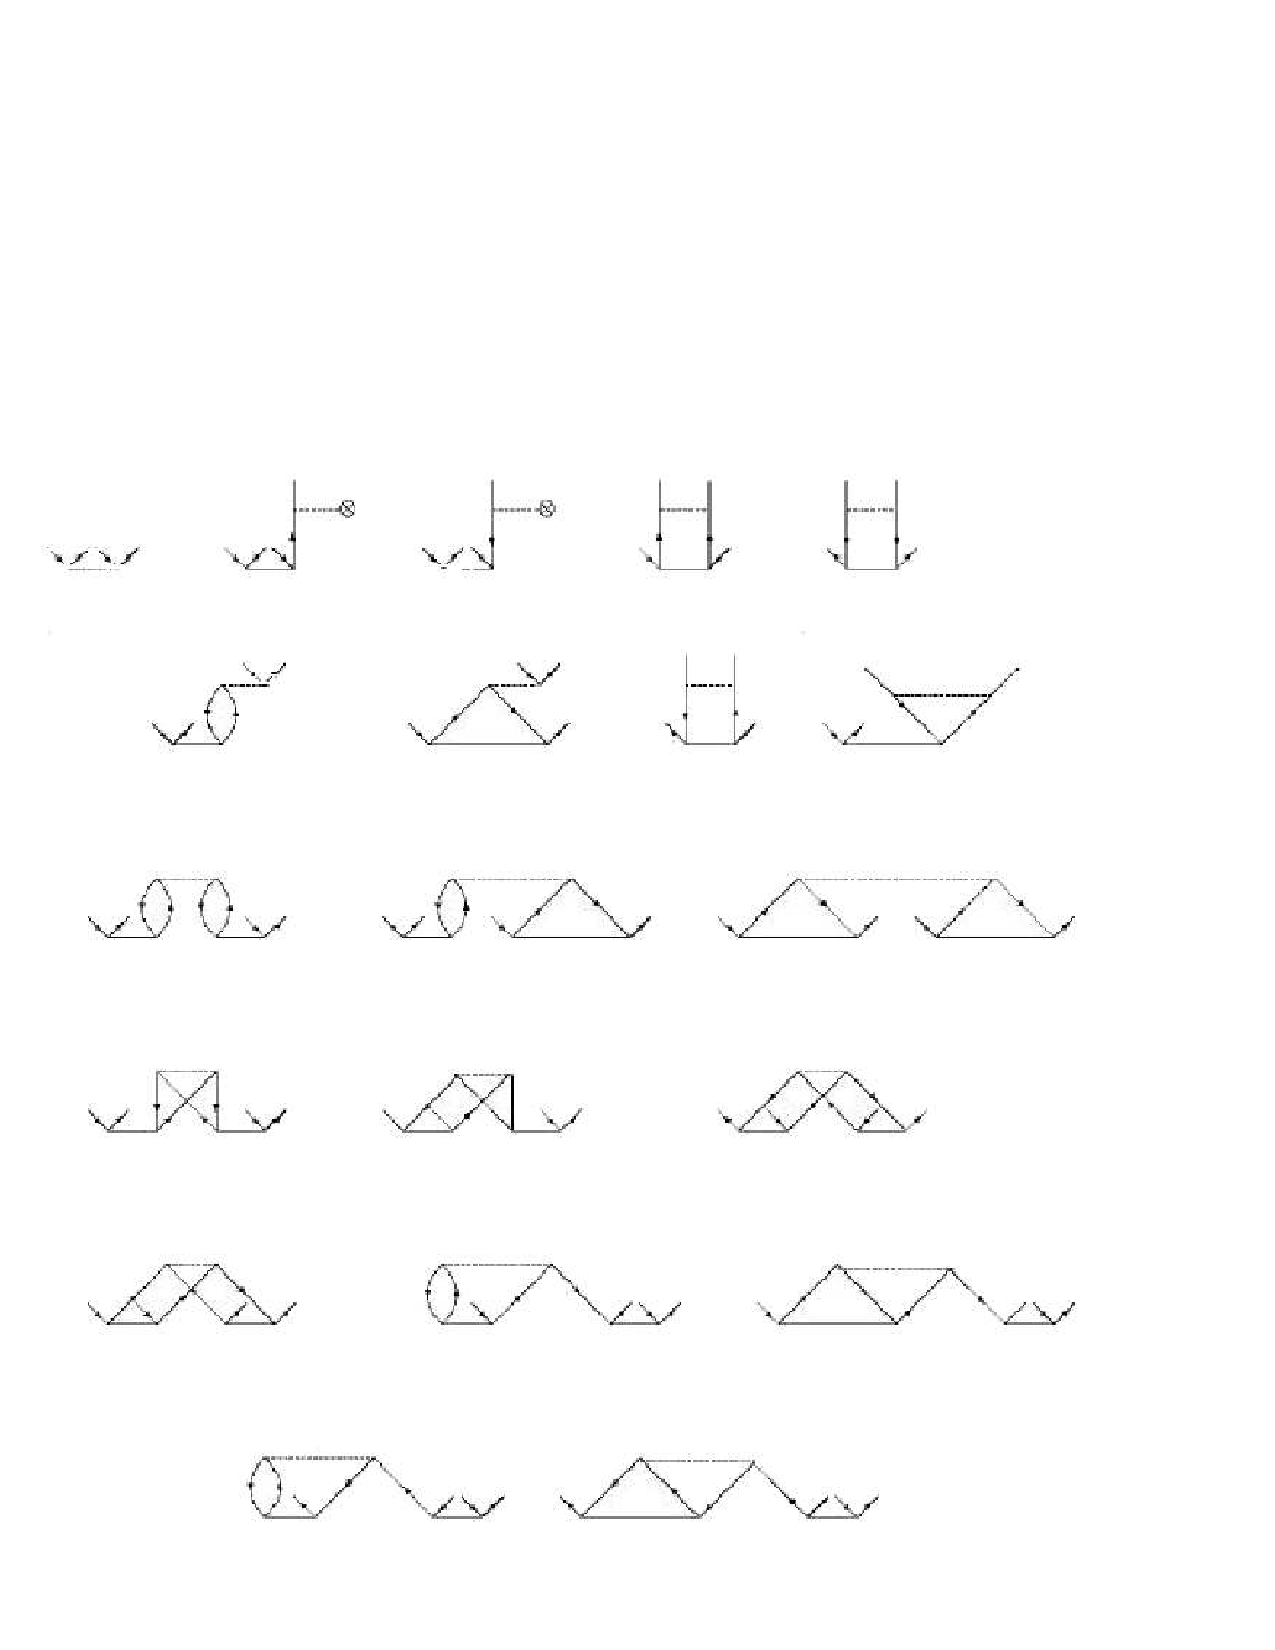
\includegraphics[scale=0.5]{CCD_diag}%{t2_eqn_diag2}
\caption{All diagrams contributing to the equation for solving the
$T_2$ amplitude.}
\label{t2_eqn_diag}
\end{figure}


\begin{figure}[htp]
\centering
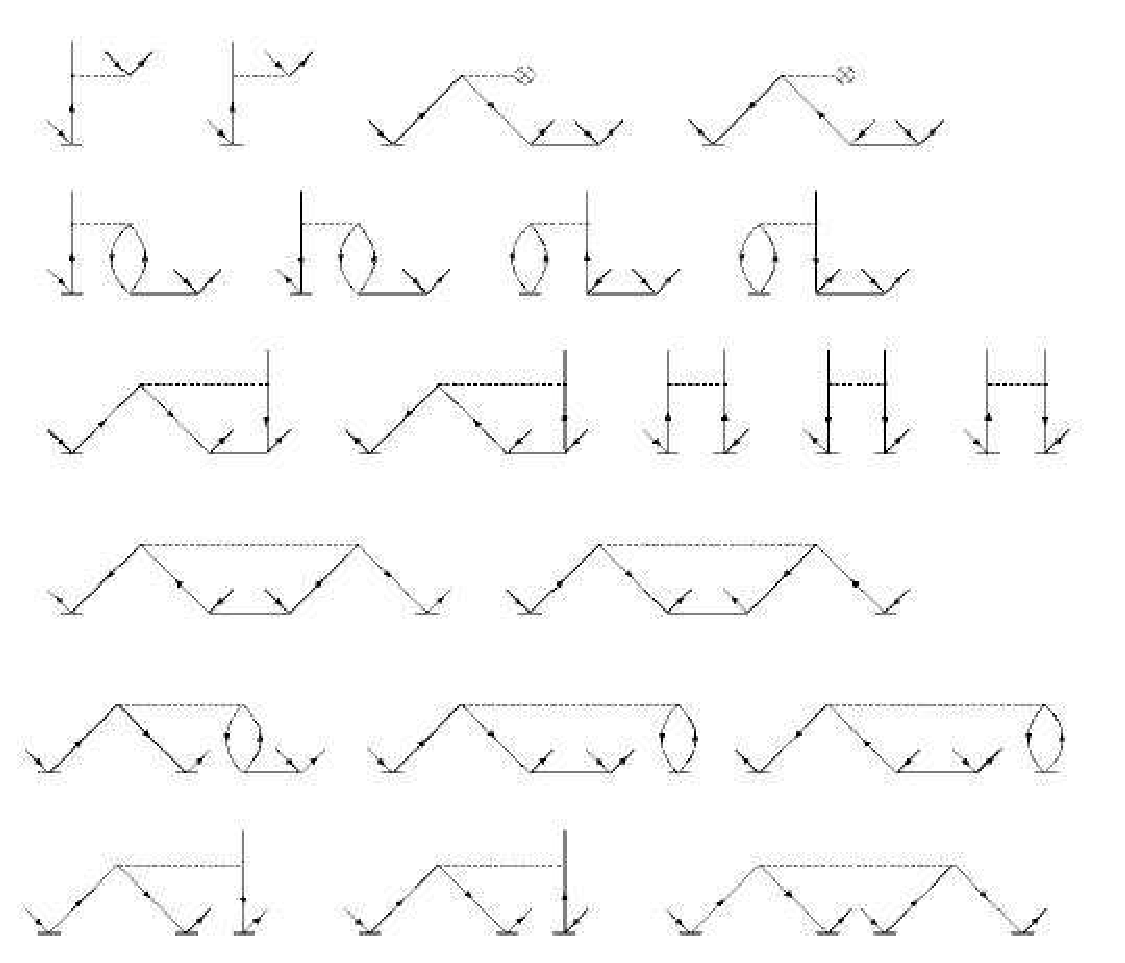
\includegraphics[scale=0.5]{CCSD_diag}%{t2_eqn_diag2}
\caption{All diagrams contributing to the equation for solving the
$T_2$ amplitude.}
\label{t2_eqn_diag}
\end{figure}


%\clearpage
To see the benefit with the diagrams, the $CCSD$ energy 
equation will now be computed from the diagrams. The total 
energy can be depicted as in Fig.(\ref{totenergydi})


\begin{figure}[htp]
\centering
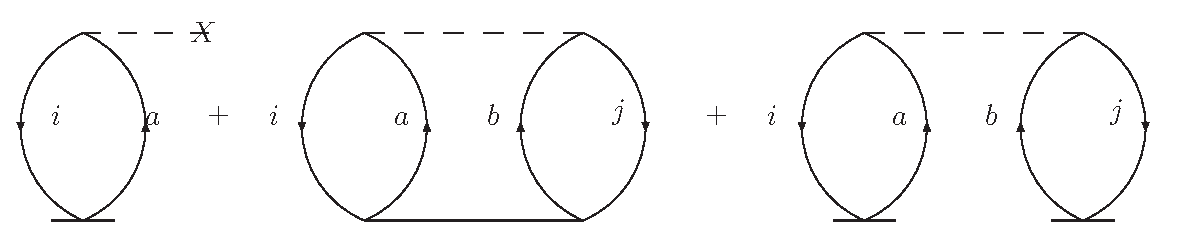
\includegraphics[width=1.0\textwidth]{energy}
\caption{The diagrams representing the total $CCSD$ 
energy.}
\label{totenergydi}
\end{figure}

The way to interpret the diagrams is from the bottom to the 
upper part, the time is upward. The ingoing states are 
represented by a ket vector and the outgoing by the dual, bra 
vector. The first figure in Fig. (\ref{totenergydi}), 
corresponding to the one particle operator should then be 
understood as

\be
\sum_{ia}\bra{i}F_N\ket{a}t^a_i=\sum_{ai}f_{ia}t^a_i,
\ee

where $f_{ia}=\bra{i}F_N\ket{a}.$ By using the above diagram 
rules to the second diagram in Fig. (\ref{totenergydi}), it's 
matrix elements become

\be
\frac{1}{4}\sum_{ijab}\bra{ij}V_N\ket{ab}t^{ab}_{ij}=\frac{1}{4}\sum_{ijab}V_{ijab}t^{ab}_{ij},
\ee

where $V_{ijab}=\bra{ij}V_N\ket{ab}.$ The last part is written 
as

\be
\frac{1}{2}\sum_{ijab}\bra{ij}V_N\ket{ab}t^a_it^b_j=\frac{1}{2}\sum_{ijab}V_{ijab}t^a_it^b_j.
\ee

After summing up the energy,  the total equation becomes

\be
\sum_{ia}f_{ia}t^a_i+\frac{1}{4}\sum_{ijab}V_{ijab}t^{ab}_{ij}
+\frac{1}{2}\sum_{ijab}V_{ijab}t^a_it^b_j,
\ee

which is exactly the same as the equation got by using Wicks 
theorem.\\ 

%The same reasoning as above for the energy equation can be done
%at the $CCSD$ amplitude equations. In this case one has to take
%in consideration that the states dealed with are excited states
%projected on the normaled ordered coupled cluster Hamiltonian 
%operated on the groundstate.
%
%The leading term in the $T_1$ amplitude  equation is $\bra{\Phi^a_i}H_N\ket{\Phi_0}$. Only the one particle operator is 
%contributing here, the corresponding diagram would be 
%
%\begin{figure}[htp]
%\centering
%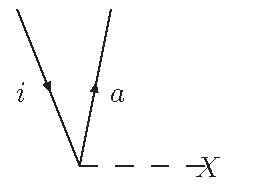
\includegraphics{firstampl}
%\caption{The diagram representing the first leading term in the
%$T_1$ amplitude equation. The interpretation is $f_{ai}$ }
%\label{firstamplt}
%\end{figure}
%
%Converting the diagram in Fig. (\ref{firstamplt}) to an equation
%would give the result $f_{ai}.$
%
%The first leading term in the $T_2$ amplitude equation is
%$\bra{\Phi^{ab}_{ij}}H_N\ket{\Phi_0},$ only the two-particle 
%operator is contributing to this part and the diagram is as is 
%shown in Fig. (\ref{secamplt})
%
%\begin{figure}[htp]
%\centering
%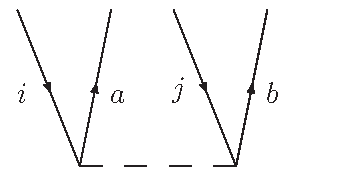
\includegraphics{secampl}
%\caption{The diagram representing the first leading term in the
%$T_2$ amplitude equation. It is representing the equation 
%$V_{ijab}$ }
%\label{secamplt}
%\end{figure}
%
%The matrix element, Fig(\ref{secamplt}), is $\bra{ab}V\ket{ij}.$


\section{Computation of the equations}

This section will treat the computational approach for solving the amplitude
equations as Eqs. \eqref{firstamplitude} and \eqref{secondamplitude}.
It is not always clear how one should approach the equations for the amplitudes. 
A first approach could be to rearrange the equations to provide a more handier form. As an example the first few terms of Eq. \eqref{firstamplitude}, could be written as

\be
0=f_{ai}+f_{aa}-f_{ii}t^a_i+\sum_c(1-\delta_{ca})f_{ac}t^c_i-\sum_k (1-\delta_{ik})f_{ik}t^a_k+\cdots
\label{firstfirstampl}
\ee

By defining 

\be
D^a_i=f_{ii}-f_{aa}
\ee

Eq. \eqref{firstfirstampl} would be rewritten as 

\be
D^a_it^a_i=f_{ai}+\sum_c(1-\delta_{ca})f_{ac}t^c_i-\sum_k(1-\delta_{ik})f_{ik}t^a_k+\cdots.
\ee

By also defining 

\be
D^{ab}_{ij}=f_{ii}+f_{jj}-f_{aa}-f_{bb}
\ee

the $T_2$ amplitude can be rewritten as

\be
D^{ab}_{ij}t^{ab}_{ij}=\bra{ab}V\ket{ij}+P(ab)\sum_c(1-\delta_{bc})f_{bc}t^{ac}_{ij}-P(ij)\sum_{k}(1-\delta_{kj})f_{kj}t^{ab}_{ik}+\cdots
\ee

The equations above have to be solved iteratively. A starting point for $t^a_i$ and $t^{ab}_{ij}$ may be obtained by setting all of the amplitudes on the right-hand side to zero. The initial guess for the amplitudes are then

\be
t^a_i=f_{ai}/D^a_i,
\ee 

for the $T_1$ amplitude and 

\be
t^{ab}_{ij}=\bra{ab}V\ket{ij}/D^{ab}_{ij}
\ee

for the $T_2$ amplitude.\\

 These initial guesses have to be inserted on the right-hand side of the 
equations and then subsequently used to obtain new 
amplitudes. This process is continued until an explicit convergence is 
reached.

We saw in Eqs. \eqref{firstamplitude} and \eqref{secondamplitude} that there
are many diagrams contributing to the amplitude equations, as many diagrams
as terms in the equations. It requires a lot of time computing all these
diagrams separately. By saving a great amount of computing time the 
amplitude diagrams are factorized. The coupled cluster diagrams can be 
factorized in contrast to the diagrams in perturbation theory since the 
first ones do not have any denominators in their's expressions. By notice 
that some diagrams are similar in the sense that they have the same factors.
Instead of computing the same factors several times, we compute it once and
multiply it with the corresponding terms, as explained by \cite{bartlett:291}. In this work the factorization used is the same as the one used by \cite{hagen:034302}.


